\documentclass[12pt]{article}

\usepackage{array} % table right-justify
\usepackage{caption}
\usepackage{changepage} % adjustwidth
\usepackage{colortbl} %
\usepackage{enumitem} %
\usepackage{xcolor}
\usepackage{float}
\usepackage{graphicx}
\usepackage{fancyhdr}
\usepackage{listings} % Code listings
\usepackage{lmodern} % better tt fonts
\usepackage{multicol}
\usepackage{multirow}
\usepackage{textcomp}
\usepackage{xurl}
\usepackage{setspace}
\usepackage{etoolbox}

\AtBeginEnvironment{quote}{\singlespacing\small}

\usepackage[utf8]{inputenc}
\usepackage{setspace}

\usepackage[dvips,letterpaper,margin=1in]{geometry}

\setlength{\parindent}{15pt}
\setlength{\headheight}{15pt} % fancyhdr wants at least 14.5pt
\setlist{noitemsep}

\definecolor{light-gray}{gray}{0.95}

% Header
\pagestyle{fancy}
\lhead{K3 Migration to Red Hat Real-Time Linux}
\rhead{September 4, 2020}
\renewcommand{\headrulewidth}{0.4pt}
\renewcommand{\footrulewidth}{0.4pt}

% Start document
\begin{document}

%%%%%%%%%%%%%%%%%%%% Title Page %%%%%%%%%%%%%%%%%%%%%%%%
\thispagestyle{empty}
\begin{titlepage}
\begin{center}
        \vspace*{1cm}

        \LARGE{Ku Band Radio Frequency System Version 3 (K3) \\
        Migration from Concurrent RedHawk Linux to \\
        Red Hat Real-Time Linux}

        \vspace{0.5cm}
        \LARGE
        % Subtitle

        \vspace{1.5cm}

        \normalsize

        John Jesus \\
        September 4, 2020

        \vfill



        \vspace{0.8cm}




\end{center}
\end{titlepage}

\tableofcontents

%%%%%%%%%%%%%%%%% Scope %%%%%%%%%%%%%%%%%%%%%%%%
%
\newpage
\section{Scope}
\subsection{Identification}
This document is a Raytheon internal document analyzing an opportunity to change
the version of Linux operating system used in the Ku Band Radio Frequency System
(KRFS) Version 3 (K3).

\subsection{System overview}
KRFS is a radar system that supports the counter- rocket, artillery, and mortar
(CRAM) mission.  KRFS has four radar apertures each operating as an Active
Electronically Scanned Array (AESA).  Each aperture has its own receiver/exciter
and signal processing subsystem called the Array Backend Electronics Unit
(ABEU).  The arrays are arranged to provide 360 degree coverage in azimuth and
horizon to 90-degree coverage in elevation.

\begin{figure}[H]
    \begin{center}
    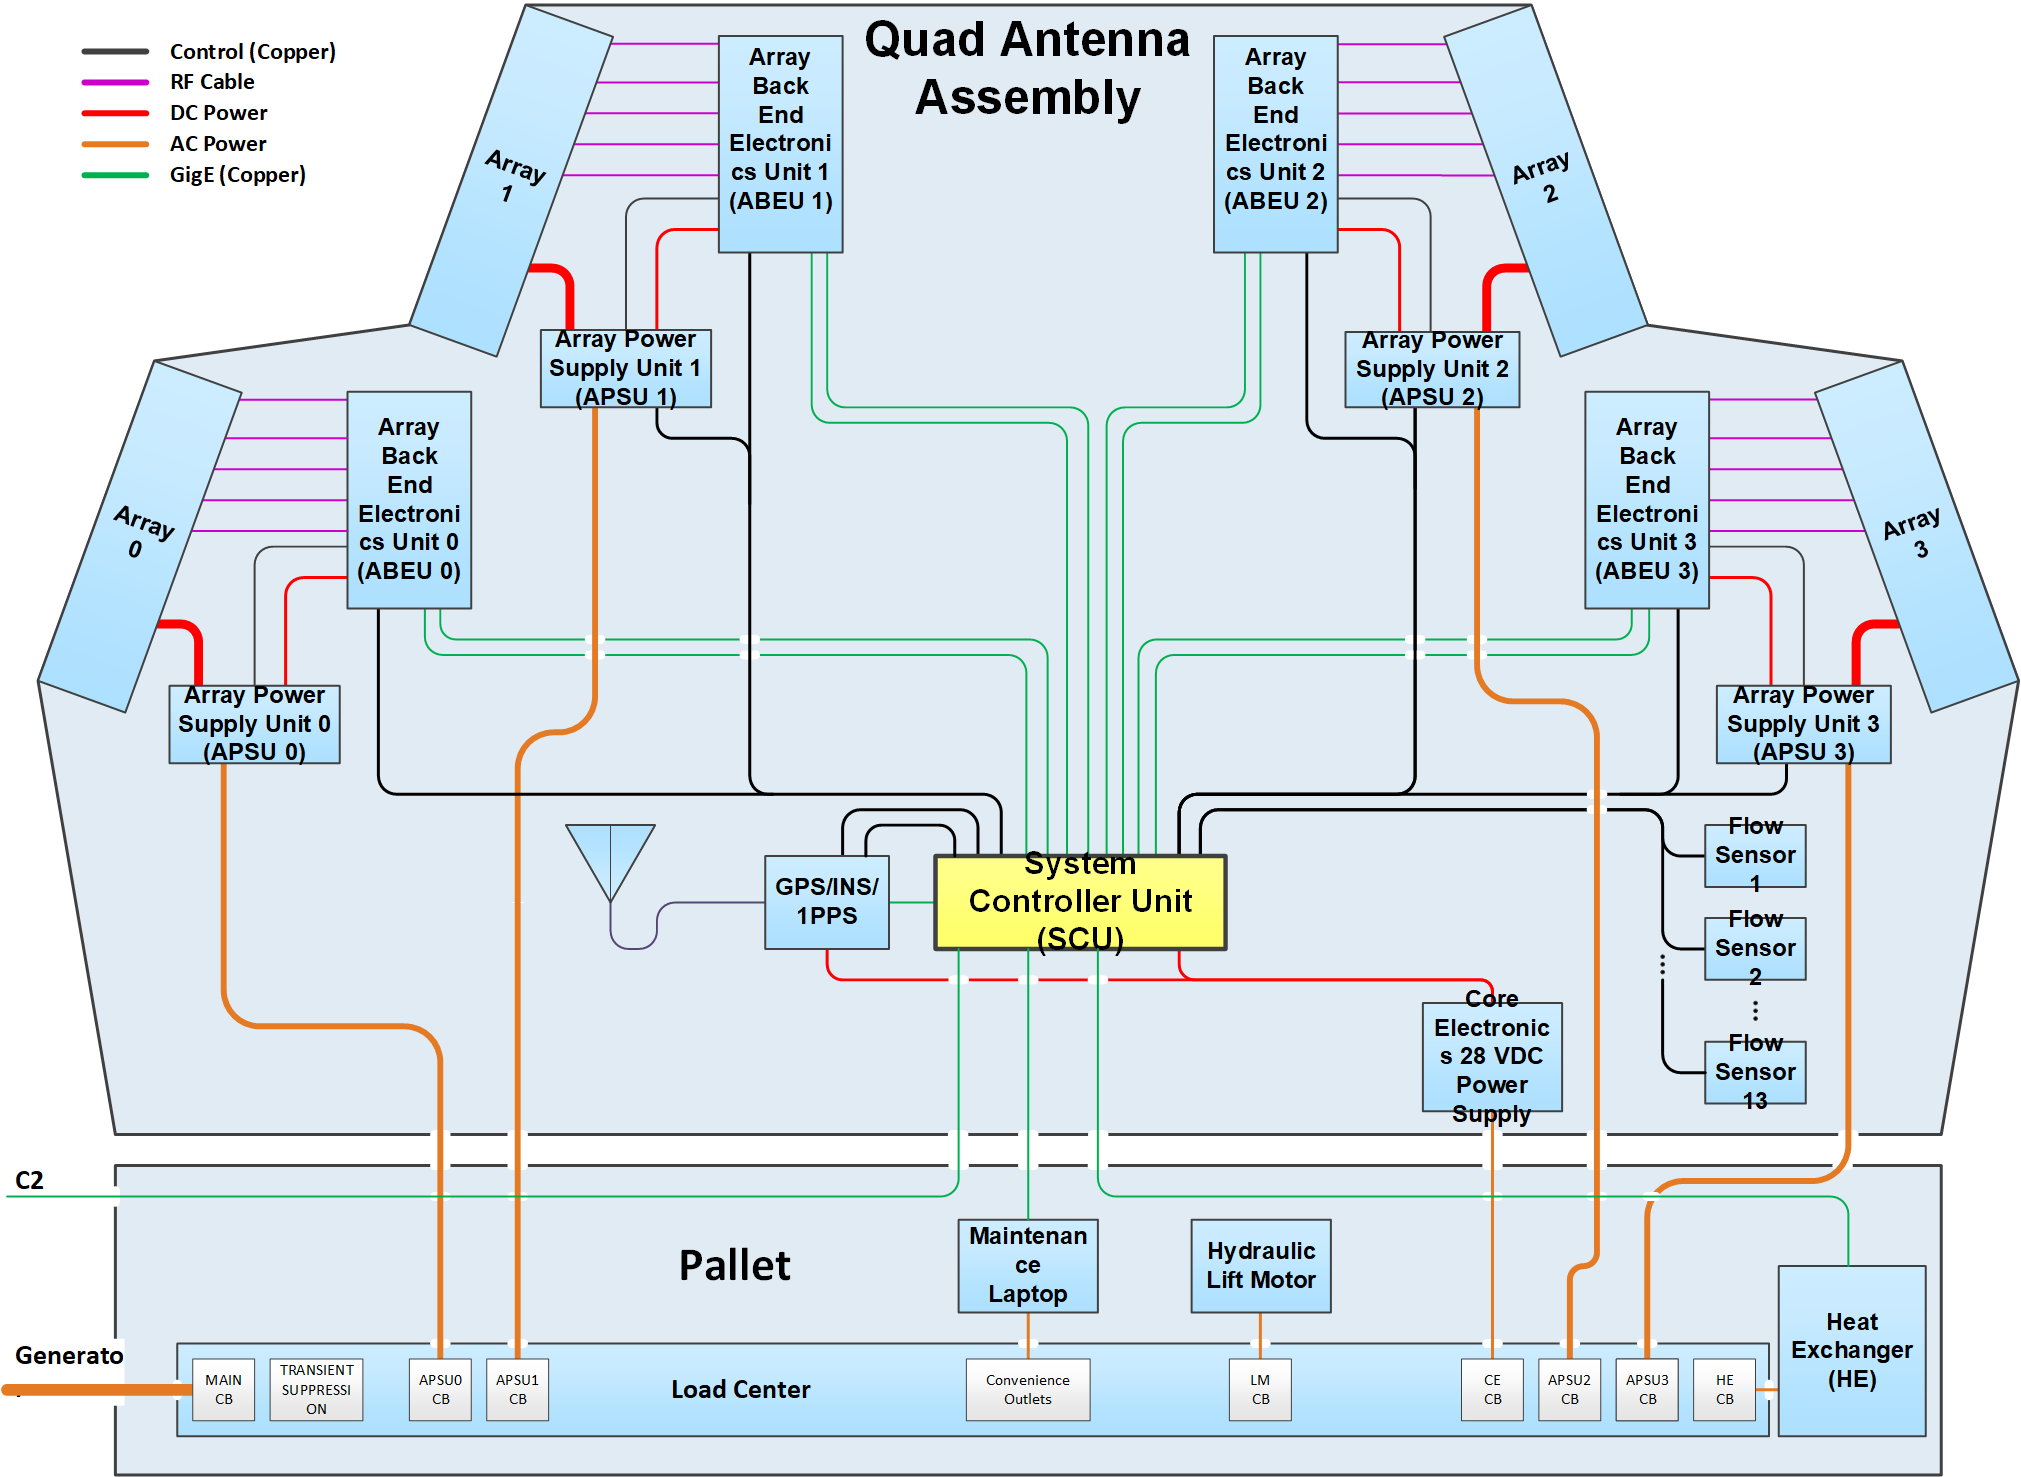
\includegraphics[width=1.0\textwidth]{img/k3}
    \caption{K3 Radar System}
    \label{fig:k3}
    \end{center}
\end{figure}

The System Controller Unit (SCU) is a 3-U VPX/VME shelf with
commercial-off-the-self (COTS) cards and one custom card assembly (CCA).  The
SCU is the central controller for the radar system, and the main control
software within the SCU runs in its SBC card (Figure \ref{fig:scu}).

\begin{figure}[H]
    \begin{center}
    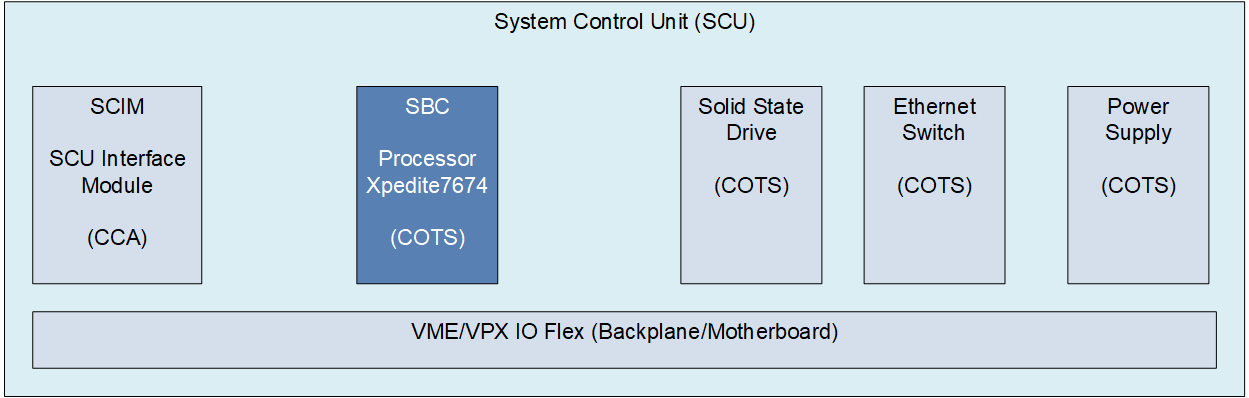
\includegraphics[width=1.0\textwidth]{img/scu}
    \caption{The SBC card in the SCU}
    \label{fig:scu}
    \end{center}
\end{figure}

In KRFS K2, the SBC Processor is a Extreme Engineering (XES) Xpedite7672 card
based on the Xeon-D System-on-a-Chip (SOC) running the Linux operating system.
In KRFS K3, the SBC Processor is a very similar Extreme Engineering (XES)
Xpedite7674 card also based on the Xeon-D SOC and running the Linux operating
system.

\subsection{Overview of Linux operating system and real-time features}
The Linux operating system is a free, open-source software (FOSS) operating
system originally authored by Linus Torvalds in September 1991 as a Unix system
for his personal computer.  Linux eventually became the operating system
underlying platforms from the smallest devices (Android phones are based on
Linux) to supercomputers. Although the source code for the software is freely
available, some commercial vendors charge fees to provide the software
pre-compiled for a particular device, board, or machine, and charge for support
and additional documentation or other tools.  Linux initially resembled the Unix
systems of its time; it supported multiple users and multiple simultaneously
running programs and used a \emph{completely fair scheduler} (CFS) to insure
equality among the running processes.

\subsubsection{Real-time patch (RT Patch) for the Linux operating system}
\label{section:rt_patch}
In the early 2000s, engineers at IBM and Red Hat were working on modifying the
Linux kernel source code to support real-time applications.  In a real-time
system like a radar, some processing has deadlines, for example, transmitting
pulses or processing signal returns, where instead of emphasizing fair
scheduling among all processes, a real-time operating system (RTOS) must assign
priorities to tasks and interrupt (preempt) not only the currently running task
but even its own internal mechanisms (spinlocks, semaphores, and interrupt
handling) to meet the real-time deadlines.  This patch was originally named
\emph{PREEMPT\_RT} or \emph{CONFIG\_PREEMPT\_RT} and authored by some of the most
important Linux kernel developers, Ingo Molnar and Thomas Gleixner of Red Hat
and Paul McKenny of IBM.  The source code for the RT Patch has been actively
maintained separately from the mainline Linux source code over the last 15 years
by teams led by these same developers and has been downloaded and incorporated
in thousands of systems and other Linux software distributions.

Some other features of the RT Patch besides kernel-level preemption:

\begin{enumerate}
\item CPU shielding - this mechanism constrains the running of operating system
threads to certain CPUs in a multicore/multiprocessor system.  KRFS uses this
feature to protect or \emph{shield} certain CPUs from running Linux kernel
lower-priority operations and lower-priority interrupts (such as disk I/O) so
that the shielded CPUs can be dedicated to real-time application (radar
processing) code.
\item CPU affinity - this mechanism enables application workload to be spread
among multiple CPUs to exploit concurrent processing.  This assignment of
application processes to \emph{cpusets} is specified in userspace (that is, the
application programmer decides this partitioning).  In KRFS, signal processing
application threads can be distributed among shielded CPUs so dedicated and
network communications can be partitioned onto other cores/CPUs.
\end{enumerate}

\subsubsection{Red Hat Real-Time Products}
The first announcement of Red Hat using their RT Patch work in their own
products was in February 2007 when IBM and Raytheon IDS of Tewksbury, MA
announced at the Boston 2007 Red Hat Summit that Red Hat real-time kernels were
running on IBM Blade Server computing clusters for the DDG 1000 Zumwalt Class
Destroyer Program.%
\footnote{https://www-03.ibm.com/press/us/en/pressrelease/21033.wss}

Later in 2007, Red Hat announced their Red Hat Messaging-Real-time-Grid (MRG)
product which bundled the real-time kernel with low-latency messaging components
and grid computing (\emph{grid computing} allows Linux to automatically spread
workload across any available CPU in a distributed cluster of machines).  In
this MRG product, Red Hat seemed to be ignoring customers who were interested in
real-time but did not need the enterprise cluster computing features, namely,
embedded systems developers.

When Red Hat released Red Hat Enterprise Linux 7 (RHEL7) in 2014, the MRG
product was deprecated, and \emph{Red Hat for Real-Time} was introduced as a
separate product.  Red Hat RT includes the standard Linux kernel with the RT
patch plus the Red Hat \emph{Tuna} tuning tool and other miscellaneous tools and
documentation, aiming this product at the embedded systems market.

\subsubsection{SuSE Linux Enterprise Real Time}
Soon after IBM and Red Hat released the original Linux RT Patch in the early
2000s, German firm \emph{Software und System-Entwicklung} (SuSE) released
\emph{SuSE Linux Enterprise Real Time} which included the RT Patch and added
some features:

\begin{enumerate}
\item Shield command - SuSE introduced a small python script to simplify the use
of the Linux \emph{cpuset} command for confining kernel and user processes to
certain processors (this script eventually moved to the main RT Patch)
\item Support for a Real-Time Clock and Interrupt Module (RCIM) - a PCI card
that provided programmable timers and 12 input and output external interrupt
lines to synchronize clocks across systems.  SuSE provided Linux device drivers
for this card.
\item A Frequency Based Scheduler (FBS) - SuSE provided a scheduler based on
the high-resolution timer provided by the RCIM to support software that
performed high-frequency short-deadline processing.  SuSE also released a
debugging tool providing a view of system utilization during each frequency
slice of the scheduler.
\end{enumerate}
\label{ref:suse_rt_features}

Although SuSE implied that they had implemented the real-time kernel features,
they were simply including the RT Patch code from Red Hat; Red Hat remarked of
the SuSE offering:

\begin{quote}
"With their latest release, (SuSE) has moved to the Red Hat-developed real-time
patch set," Che said. "If you look at it from a technology standpoint, (SuSE)
has moved to a version aligned with what Red Hat is doing. It validates our
approach that you have to work with the upstream Linux kernel." At the London
launch of MRG, line of business VP Scott Crenshaw said that (SuSE) had used beta
versions of Red Hat's code in its offering. "They haven't contributed a line of
code", he said. As a result of this change of code, he argued that "all their
prior users are cut off" from previous versions.%
\footnote{\url{http://www.internetnews.com/dev-news/article.php/3714366}}
\end{quote}


\subsubsection{Concurrent Computing Corporation RedHawk Linux}

In April 2004, Concurrent Computing Corporation announced a real-time
Linux product, containing this excerpt:

\begin{quote}
Concurrent's refinements include kernel-level priority inheritance support,
a Frequency Based Scheduler (FBS), process and IRQ shielding extensions,
user-level real-time Hyper-Treading control for Intel Xeon platforms,
user-level spin locks, significant real-time performance tuning and
many additional improvements.%
\footnote{\url{https://www.businesswire.com/news/home/20040427005101/en/Concurrent-Announces-Version-2.1-RedHawk-Real-Time-Linux}}
\end{quote}

It seems fairly obvious that this list of so-called \emph{Concurrent's refinements}
are simply features inherited from SuSE Real-Time, and, this comment from the Linux
Weekly News online was representative of many in the Linux community to
Concurrent's product announcement:

\begin{quote}
Parent article: Concurrent releases RedHawk Linux 2.1
They do not have to release source to the world, but,
they certainly do have the obligation to make source
available to those to whom they're distributing these
customized Linux kernels. The company seems to be very quiet on these
obligations, to judge from their web site. I think it's entirely
appropriate that they get some scrutiny from the folks
whose code they've customized.%
\footnote{\url{https://lwn.net/Articles/82589/}}
\end{quote}

At the same time as its repackaging of RT Patch, Concurrent released a set of
tools called \emph{NightStar} that are especially good in tracing the processing
of data as it travels between boards and over networks:

\begin{quote}
The RedHawk NightStar Tools allow users on an iHawk system running
RedHawk Linux to schedule, monitor, debug and analyze the run time behavior of
their real-time applications as well as the RedHawk Linux operating system
kernel.  The RedHawk NightStar Tools consist of the NightTrace event analyzer;
the NightSim frequency-based scheduler; the NightProbe data monitoring tool; the
NightView symbolic debugger; the NightTune system and application tuner;
shmdefine, a shared memory configuration aid tool; and the Data Monitoring API
(Datamon).  NightTrace is a graphical tool for analyzing the dynamic behavior of
single and multiprocessor applications. NightTrace can log application data
events from simultaneous processes executing on multiple CPUs or even multiple
systems. NightTrace combines application events with RedHawk Linux kernel
events, presenting a synchronized view of the entire system.  Many of the tools
include a small run-time agent that executes on the RedHawk Linux target system
in a non-intrusive manner, preserving the deterministic characteristics of the
application.%
\footnote{\emph{RedHawk NightStar Tools Version 2.2 Release Notes March 2005
0898008-2.2}, March 2005}
\end{quote}

Though the excerpt above was over fifteen years ago, the product features have
not changed, the products instead progressing by moving along with the mainline
kernel version and RT Patch and porting to new boards/platforms.

\subsubsection{Merge of RT Patch to Linux mainline in July 2019}
In July 2019, Linux Torvalds merged the RT Patch into the Linux mainline and the
latest Linux kernel can now be made real-time using a configuration option.%
\footnote{Linus Torvald's commit message is included in its entirety in Appendix
A}
This merge means that anyone can download the latest Linux kernel source and
build it to include all of the real-time features.

\subsubsection{Summary of Linux real-time options}

\begin{enumerate}
    \item Each of the real-time kernels offered from Red Hat, RedHawk, and SuSE
is the same as the others, merged from the RT Patch originally contributed and
currently maintained by Red Hat developers
    \item Though it has not changed its Red Hawk or NightStar feature set in 15
years, Concurrent's NightStar tools are very useful for distributed real-time
systems
    \item Red Hat has always had a real-time kernel product, but, it was
obscured by the enterprise cluster features with which it was packaged within
the Red Hat's MRG product, effectively hiding Red Hat's real-time kernel from
consideration by embedded systems developers.
    \item When Red Hat released Red Hat Enterprise Linux 7 (RHEL7) in 2014, the
MRG product was deprecated, and \emph{Red Hat for Real-Time} was introduced as a
separate product.  Red Hat RT includes the standard Linux kernel with the RT
patch plus the Red Hat \emph{Tuna} tuning tool and other miscellaneous tools and
documentation, aiming this product at the embedded systems market.
    \item The RT Patch was merged into the Linux Kernel mainline in July 2019
and thus available to anyone who downloads and builds the kernel source code
\end{enumerate}



\subsection{Document purpose}
%To integrate NE software, we need to be able to build Linux from source.  NE
%currently uses Red Hat Real-Time.  We use Red Hawk from Concurrent RTI.  NE
%builds from source using tools from Red Hat.  We do not build from source.
%
%Produce a document that helps us decide how to get our Linux image created.


\subsection{Document overview}
The structure of this document:

\begin{enumerate}
    \item Document scope (this section)
    \item References
    \item Real-time features from RedHawk used in current KRFS software
    \item Creating the Linux operating system image
    \item Hardening the Linux operating system image
    \item Migrating to Red Hat Real-Time in K3
\end{enumerate}



%%%%%%%%%%%%%%%%% References %%%%%%%%%%%%%%%%%%%%%%%%
%
\newpage
\section{References}

\begin{enumerate}
    \item \textit{RedHawk Linux Users Guide 0898004-780} (Concurrent Computer
Corporation, March 2016) \label{ref:red_hawk_guide}
    \item \textit{RedHawk Architect Users Guide 0898601-7.2-1} (Concurrent
Computer Corporation, December 2016) \label{ref:architect}
    \item \textit{NightStar RT Tutorial Version 4.4 0898009-090} (Concurrent
Computer Corporation, May 2014) \label{ref:nightstar}
    \item \textit{Red Hat Enterprise Linux for Real Time 7 Reference Guide} (Red
Hat Corporation, November 6, 2015) \label{ref:rhel7_ref}
    \item \textit{Red Hat Enterprise Linux for Real Time 7 Installation Guide}
(Red Hat Corporation, November 6, 2015) \label{ref:rhel7_install}
    \item \textit{Preboot Execution Environment (PXE) Specification Version 2.1}
(Intel Corporation, September 20, 1999) \label{ref:pxe_boot}
    \item Source for Red Hawk costs in Table \ref{tab:license_costs} was Karl
Weis, Global Supply Chain Program Lead, Raytheon \label{ref:karl}
    \item Source for Red Hat Real-Time costs in Table \ref{tab:license_costs}
was Lynn Bonenfant, IT Program Lead, Raytheon \label{ref:lynn}
    \item \textit{Pull CONFIG\_PREEMPT\_RT stub config from Thomas Gleixner}
commit message from the web view of the Linux git repository at
\url{https://git.kernel.org/pub/scm/linux/kernel/git/torvalds/linux.git/commit/?id=70e6e1b971e46f5c1c2d72217ba62401a2edc22b}
\label{ref:commit}
\end{enumerate}


%%%%%%%%%%%%%%%%% RedHawk Features %%%%%%%%%%%%%%%%%%%%%%%%
%
\newpage
\section{Real-time features from RedHawk in KRFS}
\label{sec:redhawk_features}

KRFS presently is on the Concurrent RedHawk Linux platform. Table
\ref{tab:redhawk_features_1} and Table \ref{tab:redhawk_features_2} list the
Concurrent RedHawk features in the order they appear in Reference
\ref{ref:red_hawk_guide} even though not all of the features are actually
real-time Linux kernel features; for example, hyper-threading is a hardware
setting in Intel CPU and the RCIM card is a piece of hardware and the XFS
filesystem originally from SGI is technically outside the kernel.  All of the
real-time kernel features are inherited from the RT Patch described in Section
\ref{section:rt_patch} except for those based on the RCIM card (device driver,
scheduler, process accounting).

Only the first two features from the list are explicitly used by KRFS source
code.

\begin{table}[H]
    \captionsetup{width=.9\linewidth}
    \caption{RedHawk real-time feature list (Part 1)}
    \resizebox{\textwidth}{!}{%
    \begin{tabular}{p{2.8in}p{1.2in}p{3.6in}}
    \hline
        \textbf{Feature} & \textbf{Used in KRFS} & \textbf{Description} \\
    \hline
        \rowcolor{light-gray} Processor Shielding & \textbf{Yes} & KRFS
currently uses the old syntax from SuSE and Concurrent \emph{shield} instead of
the now-standard Linux command \emph{cset} \\
        \rowcolor{light-gray} Processor Affinity & \textbf{Yes} & KRFS code
uses the POSIX thread interface to set processor affinity \\[4.5mm]
User-level Preemption Control & No & User control of preemption of userspace
synchronization mechanisms like POSIX semaphores using a system function call
\emph{resched\_cntl}.  Makes kernel space preemption mechanism invocable from
userspace. \\
Fast Block/Wake Services & No & A preemptible semaphore in the kernel available
from RT Patch since 2007. \\
RCIM Driver & No & Concurrent sells a PCI card called the Real-time Clock
Interface Module (RCIM).  The card can provide a 400ns clock signal to the
operating system through an interrupt handler to enable a high-resolution timer
feature. \\
Frequency-Based Scheduler (FBS) & No & Source code for the FBS provided by
Concurrent is actually copied without attribution from the original SuSE Linux
Real-Time Extensions released in 2006. \\
/proc Modifications & No & This feature is part of the \emph{usermap} feature
(see below) that can be used by NightStar or even regular users.\\
Kernel Trace Facility & No & This feature is combined with the standard kernel
debuggers to support enhanced kernel debugging features using NightStar \\
ptrace Extensions & No & This feature is combined with the \emph{usermap}
feature (below) to support NightStar debugging) \\
    \hline
    \end{tabular}%
    }
    \label{tab:redhawk_features_1}
\end{table}


\begin{table}[H]
    \captionsetup{width=.9\linewidth}
    \caption{RedHawk real-time feature list (Part 2)}
    \resizebox{\textwidth}{!}{%
    \begin{tabular}{p{2.8in}p{1.2in}p{3.6in}}
    \hline
        \textbf{Feature} & \textbf{Used in KRFS} & \textbf{Description} \\
    \hline
Kernel Preemption & (Yes,built-in) & Kernel Preemption is from the RT Patch \\[4.5mm]
Real-Time Scheduler & (Yes,built-in) & Alternatives to the Linux default
Completely Fair Scheduler (CFS) like priority-based SCHED\_FIFO and SCHED\_RR
(round-robin) have been part of the RT Patch since 2007.  SCHED\_DEADLINE is
available in Linux 3.6 (Red Hat 7.6) and later. \\[4.5mm]
Low Latency Enhancements & (Yes,built-in) & Some kernel tuning configuration
have been compiled in as defaults. \\[4.5mm]
Priority Inheritance & (Yes,built-in) & From the RT Patch. \\[4.5mm]
High Resolution Process Accounting & No & This feature follows from the use of
the RCIM card and driver (above).\\[4.5mm]
Capabilities Support & No & Permission files (\emph{capabilities} files) for
features like the \emph{usermap} and \emph{/proc mmap} features (below).
\\[4.5mm]
Kernel Debuggers & (Yes,built-in) & The built-in kernel debuggers \emph{kdb} and
\emph{kgdb} can be configured to work with NightStar. \\[4.5mm]
Kernel Core Dumps/Crash and Live Analysis & (Yes,built-in) &  This feature
supports NightStar, allowing it to directly map and introspect kernel memory.
\\[4.5mm]
User-level Spin Locks & No &  User control of preemption of spinlocks in the
kernel provided by a special system function call \emph{resched\_cntl}.  Makes
kernel space preemption mechanism invocable from userspace. \\[4.5mm]
usermap and /proc mmap & No & This feature supports NightStar, allowing it to
directly map and introspect any user process.  \\[4.5mm]
Hyper-threading & (Yes,built-in) & This is a setting in the CPU hardware that is
controlled in the BIOS or bootloader that allows in-core multi-processing.
Support in mainline Linux for hyper-threading and symmetric multi-processing
(SMP) has been since 2004.  \\[4.5mm]
XFS Journaling File System & (Yes,built-in) & %
The XFS filesystem was invented at Silicon Graphics (SGI) in 1996 and has been
available for mainline Linux since 2001.%
\\
    \hline
    \end{tabular}%
    }
    \label{tab:redhawk_features_2}
\end{table}

\subsection{KRFS source code changes for a non-RedHawk Linux}

\subsubsection{Shielding CPUs from low-priority system tasks}

CPUs can be shielded from the kernel command-line by using the \emph{isolcpus}
kernel boot parameter to specify one or more CPUs to isolate from the general
Linux kernel scheduler algorithms (Listing \ref{lst:shield_kernel}).


\vspace{0.8cm}
\lstset{
    language=bash,
    basicstyle=\footnotesize\ttfamily,
    linewidth=6in,
    frame=single,
    showstringspaces=false,
    keywordstyle=\ttfamily
}
\begin{minipage}{\linewidth}
\begin{adjustwidth}{0.0in}{0.0in}
\begin{lstinputlisting}[caption={Shielding CPUs at at kernel boot command-line},
label={lst:shield_kernel}]{bootparam.sh}

\end{lstinputlisting}
\end{adjustwidth}
\end{minipage}
\vspace{0.8cm}

To shield CPUs anytime after kernel boot the \emph{cset} command can be used
(Listing \ref{lst:shield_cmd}).

\vspace{0.8cm}
\lstset{
    language=bash,
    basicstyle=\footnotesize\ttfamily,
    linewidth=6in,
    showstringspaces=false,
    keywordstyle=\ttfamily
}
\begin{adjustwidth}{0.0in}{0.0in}
\begin{lstinputlisting}[caption={Shielding CPUs at command-line},
label={lst:shield_cmd}]{shield.sh}

\end{lstinputlisting}
\end{adjustwidth}
\vspace{0.8cm}

\subsubsection{CPU affinity for processes and threads}

To pin a process onto a particular cpu or cpuset, instead of using the RedHawk
\emph{run} command, use the standard \emph{taskset} command.

\vspace{0.8cm}
\lstset{
    language=bash,
    basicstyle=\footnotesize\ttfamily,
    linewidth=6in,
    showstringspaces=false,
    keywordstyle=\ttfamily
}
\begin{adjustwidth}{0.0in}{0.0in}
\begin{lstinputlisting}[caption={Use taskset instead of run},
label={lst:taskset_cmd}]{taskset.sh}

\end{lstinputlisting}
\end{adjustwidth}
\vspace{0.8cm}

KRFS source code already uses the POSIX \emph{pthreads} to set affinity for
threads, either in the thread attributes object used at thread creation or using
the functions \emph{pthread\_setaffinity\_np()} or
\emph{pthread\_attr\_setaffinity\_np()}.%
\footnote{\url{https://man7.org/linux/man-pages//man3/pthread_attr_setaffinity_np.3.html}}


%%%%%%%%%%%%%%%%% Image creation %%%%%%%%%%%%%%%%%%%%%%%%
%
\newpage
\section{Creating the Linux operating system image}
\label{sec:image_creation}

%%%%%%%%%%%%%%%%% RedHawk boot in K2 %%%%%%%%%%%%%%%%%%%%%%%%

\subsection{RedHawk Boot in K2}

\subsubsection{Normal Boot with RedHawk in K2}
The normal boot of RedHawk Linux in K2 is depicted in Figure \ref{fig:normal_boot}.
On reset, the Xeon-D jumps into the boot flash (bottom of diagram) where two
components called CoreBoot and SeaBIOS are installed; both CoreBoot and SeaBIOS
come not from RedHawk but from the board vendor X-ES.  The Xeon-D begins
booting CoreBoot (Item 1) and CoreBoot subsequently loads its payload called
SeaBIOS which is a small piece of software that decides the Linux boot method
(Item 2).

The RedHawk Linux kernel is in the local SSD flash (upper-right of diagram) on
the 7672 with a Linux root filesystem.  SeaBIOS accesses the Master Boot Record
(MBR) in the local SSD flash (upper-right) and checks for a magic number at the
end which was previously inserted by KRFS software (Item 3).  The magic number
is an indicator that the local SSD contains the normal boot contents, and,
SeaBIOS continues to boot from the local SSD if it finds the magic number there;
if the magic number is not found, SeaBIOS will advance to the next boot option,
which is a network boot over Ethernet (Item 4).

\begin{figure}[H]
    \begin{center}
    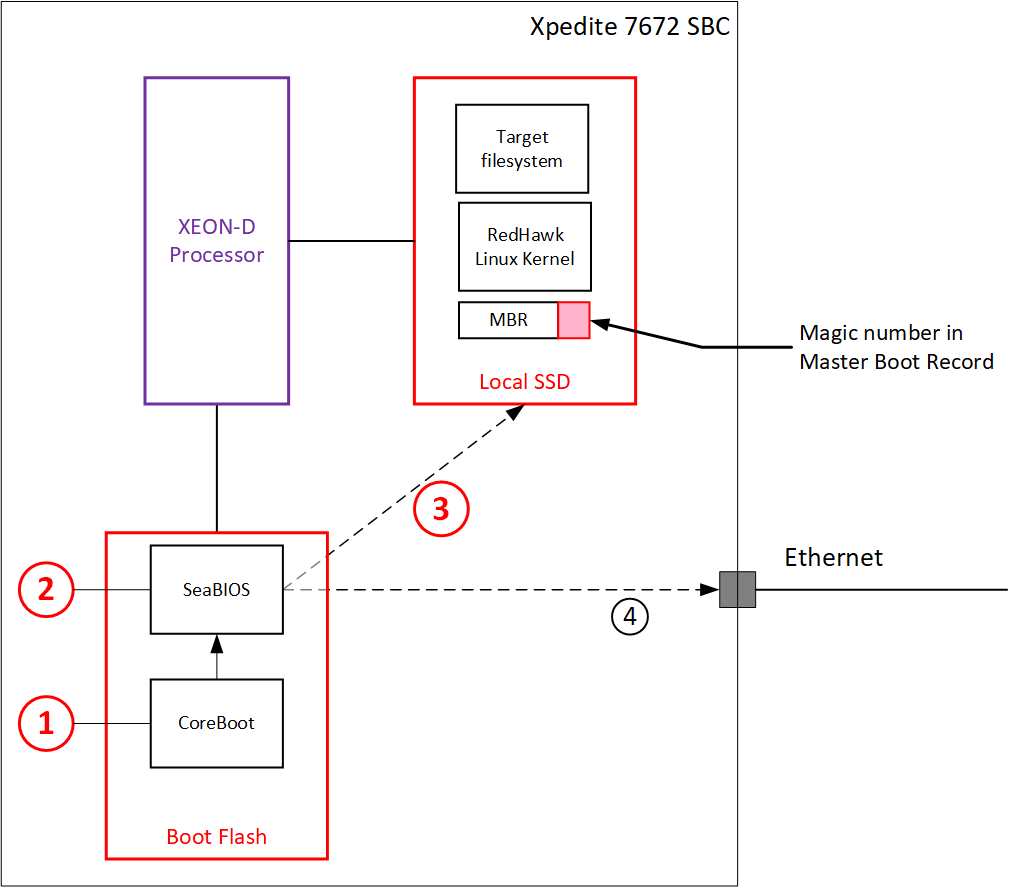
\includegraphics[width=0.6\textwidth]{img/normal_boot}
    \caption{Normal boot of SBC with RedHawk in K2}
    \label{fig:normal_boot}
    \end{center}
\end{figure}

\subsubsection{PXE Boot to Install RedHawk in K2}
To install RedHawk onto the local SSD flash, a technique depicted
in Figure \ref{fig:pxe_install} combines a network boot (called \emph{PXE Boot})
with an embedded installation script.  A full description of PXE Boot is in
Reference \ref{ref:pxe_boot}.

To force a PXE boot, the magic number in the Master Boot Record of the local SSD
(upper-right of diagram) is invalidated.  Erasing the SSD will also invalidate the
MBR as will using a special KRFS tool to erase the magic number.  With the MBR
magic number invalidated, when the system is rebooted, SeaBIOS will detect that
local SSD is not bootable (Item 3) and will advance to the next boot option
which is a PXE Boot (Item 4).  SeaBIOS will broadcast PXE boot requests on the
Ethernet which will be detected and serviced by a maintenance laptop plugged
into the same Ethernet network (Item 5).  The laptop provides a small Linux
kernel image (called \emph{vmlinuz}) and a tiny root file system (called an
initial ramdisk or \emph{initrd.img}) over the network which SeaBIOS loads into
RAM and then has the Xeon-D jump into this Linux kernel in RAM (Item 6).
Embedded within the initial ramdisk is an installation script, which pulls a
tarball called \emph{image.tgz} from the laptop and installs it onto the local
SSD (Item 7).  This tarball contains the tactical RedHawk Linux Kernel and root
filesystem.  After a successful install, the installation script inserts the
magic number into the Master Boot Record and the local SSD is ready to be
booted.  The next time the system boots, SeaBIOS will detect that a good image
is installed in the local SSD and boot from it.

\begin{figure}[H]
    \begin{center}
    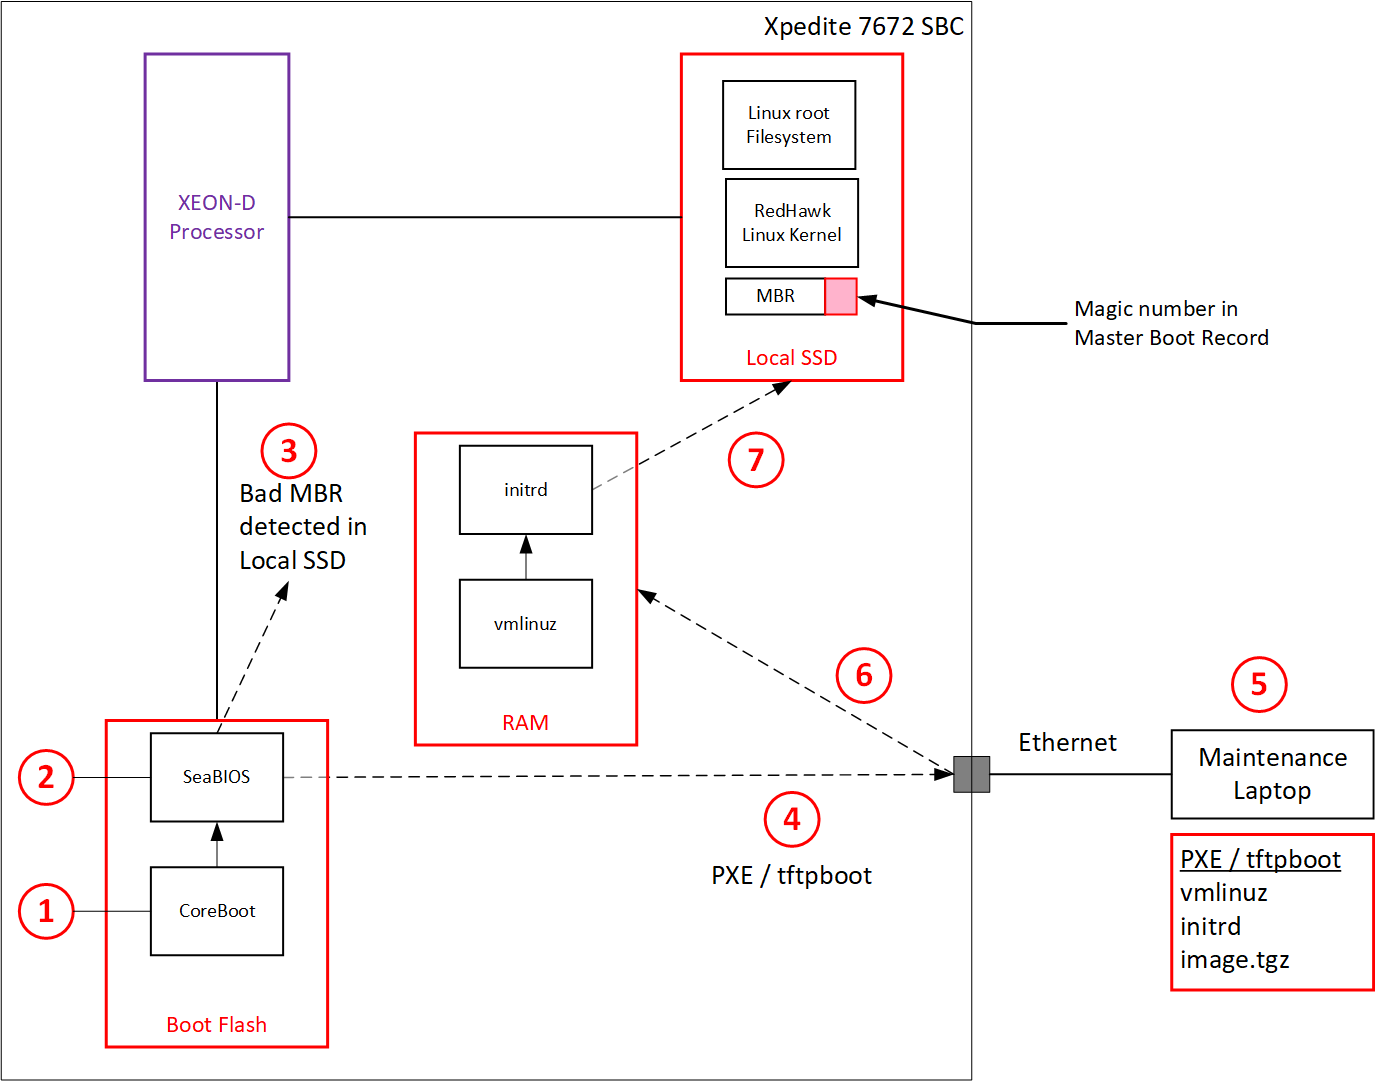
\includegraphics[width=0.8\textwidth]{img/pxe_install}
    \caption{PXE Install of SBC with RedHawk in K2}
    \label{fig:pxe_install}
    \end{center}
\end{figure}

%
\subsection{RedHawk Architect in K2}
RedHawk provides a build system called Architect to build the artifacts of Figure
\ref{fig:pxe_install}. RedHawk Architect requires an entire Red Hat Linux
machine dedicated to host it as depicted in Figure \ref{fig:architect_host}. A
dedicated host is required because as stated in Chapter 11 of Reference
\ref{ref:red_hawk_guide}:

\begin{quote}
It is often necessary to build driver modules for use with either one of the pre-existing
kernels supplied by Concurrent Real-Time or a custom kernel.
To build driver modules for a kernel, the following conditions must be met:

\textbf{The desired kernel must be the currently running kernel.}

The -c option to ccur-config can be used to ensure that the kernel source
directory is properly configured. This option automatically detects the running
kernel and configures the source tree to properly match the running kernel.
Driver modules can then be properly compiled for use with the running kernel.
\end{quote}

The KRFS Linux device drivers and scripts are copied onto this machine and are
built against the RedHawk kernel headers and RedHawk kernel libraries.

\begin{figure}[H]
    \begin{center}
    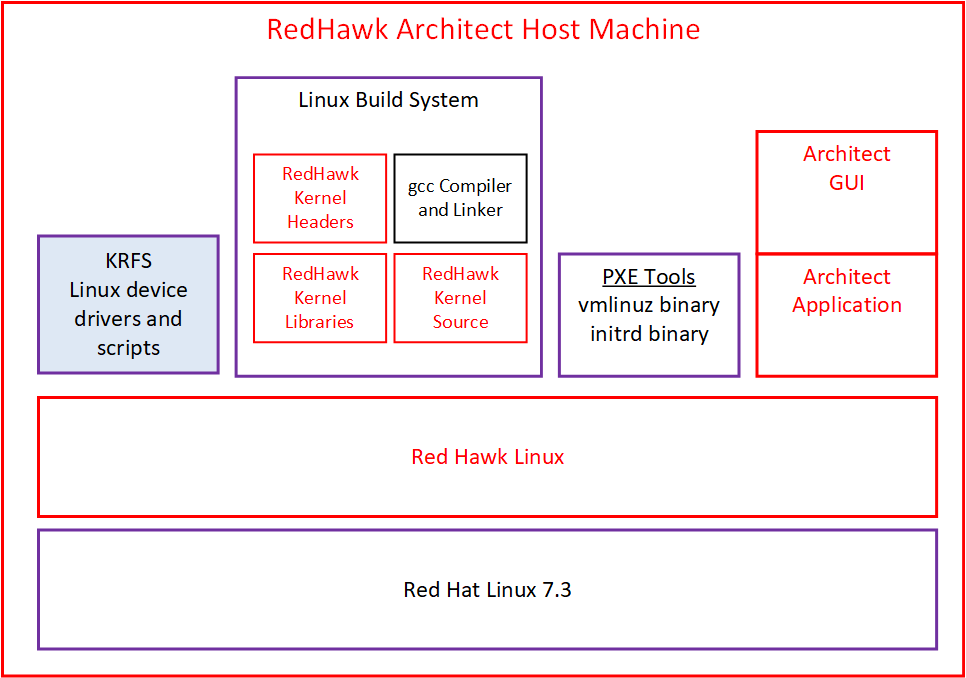
\includegraphics[width=0.8\textwidth]{img/architect_host}
    \caption{RedHawk Architect host machine}
    \label{fig:architect_host}
    \end{center}
\end{figure}

The build is invoked from a privileged user from the Architect GUI (Figure
\ref{fig:architect_screenshot}) to produce the build artifacts specified in Table
\ref{tab:architect_artifacts}.

\begin{figure}[H]
    \begin{center}
    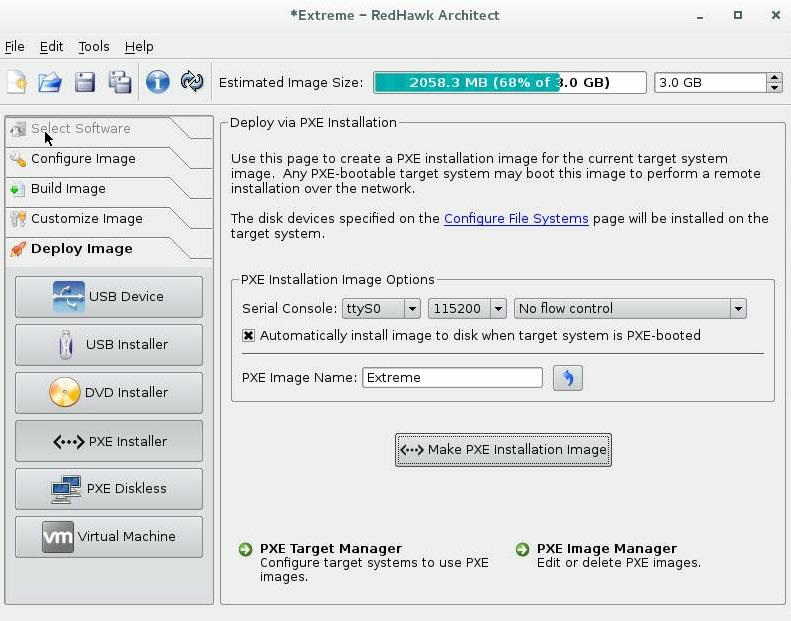
\includegraphics[width=1.0\textwidth]{img/architect_screenshot}
    \caption{Screenshot from the RedHawk Architect Tool}
    \label{fig:architect_screenshot}
    \end{center}
\end{figure}

\begin{table}[H]
    \captionsetup{width=1.0\linewidth}
    \caption{Artifacts created with RedHawk Architect}
    \resizebox{1.0\textwidth}{!}{%
    \begin{tabular}{%
    >{\raggedright\arraybackslash}p{1.6in}%
    >{\raggedright\arraybackslash}p{2.8in}%
    >{\raggedleft\arraybackslash}p{1.0in}}
    \hline
                            & \textbf{Artifact Name} & \textbf{Size (MB)} \\
    \hline
        PXE Boot files      &  & \\
                            & vmlinuz                &     5.3 \\
                            & initrd.img             &     7.0  \\
                            & other PXE config files & $ < 1.0$  \\
    \hline
        Target system image &  & \\
                            & image.tgz                    & 700.0  \\
                            & partition info, fstab, other %
                              config files               & $ < 1.0$  \\
    \hline
    \end{tabular}%
    }
    \label{tab:architect_artifacts}
\end{table}

The artifacts are then installed into the tftpboot area of the Maintenance
Laptop so that they can be installed using the PXE Boot mechanism of Figure
\ref{fig:pxe_install}.


%%%%%%%%%%%%%%%%% DevSecOps in K3 %%%%%%%%%%%%%%%%%%%%%%%%
%
\subsection{DevSecOps Linux in K3}

\subsubsection{Compiling the Linux kernel from source}

\subsubsection{XES BSP kernel objects}

\subsubsection{KRFS kernel objects and device drivers}

\subsubsection{DevSecOps deployment in K3}



%%%%%%%%%%%%%%%%% Hardening %%%%%%%%%%%%%%%%%%%%%%%%
%
\newpage
\section{Hardening the Linux operating system}
\label{sec:image_hardening}

To harden an operating system is to minimize vulnerabilities to malicious
outside access; for example, requiring a password for login is a basic hardening
mechanism.

The Defense Information Systems Agency (DISA) publishes guidance for hardening
specific operating systems called Security Technology Implementation Guidance
(STIG).  For Linux distributions, DISA publishes a STIG for only these Linux
Distributions:
\begin{enumerate}
    \item Red Hat Linux
    \item Oracle Linux
    \item SuSE Linux
\end{enumerate}

The STIG is published in an unconventional format: as an XML file.  An excerpt
from the \emph{Red Hat Enterprise Linux 7 STIG} is in Appendix B.  The XML file
contains hundreds of elements each specifying a security item to be checked
and even contains instructions for remedying the item.  This XML file can be
parsed by tools that generate reports or maintain a vulnerability database.

A different government agency National Institute of Standards and Technology
(NIST) publishes the DISA STIG in a slightly different XML format called
Security Content Automation Protocol (SCAP) that provides a better interface for
security tools that check systems and generate reports or even automate the
remedies.  The most popular open-source SCAP tool is OpenSCAP and the most used
SCAP tool in the defense community is the SCAP Compliance Checker (SCC) from
Space and Naval Warfare Systems Center (SPAWAR).

\subsection{Hardening with home-grown bash scripts in K2}
On KRFS K2, the SPAWAR SCC tool is installed onto an SBC card running an initial
Linux image released from KRFS.  The SCC tool is invoked to produce a report
listing any vulnerabilities and assigning a score to the Linux image on that
card.  KRFS source code includes bash scripts whose content is extracted from
the STIG or SCAP files, and, these bash scripts are run on the SBC card to
execute the STIG-prescribed remedies.  The SPAWAR SCC tool is run again to
produce another report and score, and, this process repeats until an acceptable
security posture is achieved.  This hardened Linux filesystem image is then
captured and becomes the new master Linux image.

\subsection{Using DevSecOps tools for hardening in K3}
For the Linux image produced for K3, instead of using the home-grown bash
scripts to apply the STIG remedies, a DevSecOps
tool\footnote{https://github.com/ansible-lockdown/RHEL7-STIG} based on
Ansible\footnote{https://www.ansible.com/} (now part of Red Hat) will be used to
automatically harden the operating system as part of the DevSecOps build-deploy
process.

%%%%%%%%%%%%%%%%% Migrating to Red Hat %%%%%%%%%%%%%%%%%%%%%%%%
%
\newpage
\section{Migrating to Red Hat Real-Time in K3}
\label{sec:redhat_migration}

\subsection{Source code changes}

\subsection{Build artifact changes}

\subsection{License costs}

Table \ref{tab:license_costs} summarizes license costs (see References
\ref{ref:karl} and \ref{ref:lynn}).

\begin{table}[H]
\captionsetup{width=.9\linewidth}
\caption{License costs}
\resizebox{\textwidth}{!}{%
\begin{tabular}{%
    >{\raggedright\arraybackslash}p{3.2in}%
    >{\raggedleft\arraybackslash}p{1.0in}%
    >{\raggedleft\arraybackslash}p{1.0in}}
\hline
                                 & Red Hawk & Red Hat RT \\
\hline
    Product Maintenance (yearly) & 281,000 & 0 \\
    Development License (yearly) &  20,796 & 2,700 \\
\hline
    Run-time License (perpetual, per-instance) & 300 & 0 \\
    Run-time License (yearly, per-instance) & 400 & 2,700 \\
\hline
\end{tabular}%
}
\label{tab:license_costs}
\end{table}


%%%%%%%%%%%%%%%%% Appendix A: Merge of RT Patch to mainline %%%%%%%%%%%%%%%%%%%%
%
\newpage
\section{Appendix A: July 2019 Merge of RT Patch to Linux mainline}

The git commit message from Linus Torvalds merging the real-time patch
into the Linux mainline on July 20, 2019 is below (Reference \ref{ref:commit}).

\begin{verbatim}
Pull CONFIG_PREEMPT_RT stub config from Thomas Gleixner:
 "The real-time preemption patch set exists for almost 15 years now and
  while the vast majority of infrastructure and enhancements have found
  their way into the mainline kernel, the final integration of RT is
  still missing.

  Over the course of the last few years, we have worked on reducing the
  intrusivenness of the RT patches by refactoring kernel infrastructure
  to be more real-time friendly. Almost all of these changes were
  benefitial to the mainline kernel on their own, so there was no
  objection to integrate them.

  Though except for the still ongoing printk refactoring, the remaining
  changes which are required to make RT a first class mainline citizen
  are not longer arguable as immediately beneficial for the mainline
  kernel. Most of them are either reordering code flows or adding RT
  specific functionality.

  But this now has hit a wall and turned into a classic hen and egg
  problem:

     Maintainers are rightfully wary vs. these changes as they make only
     sense if the final integration of RT into the mainline kernel takes
     place.

  Adding CONFIG_PREEMPT_RT aims to solve this as a clear sign that RT
  will be fully integrated into the mainline kernel. The final
  integration of the missing bits and pieces will be of course done with
  the same careful approach as we have used in the past.

  While I'm aware that you are not entirely enthusiastic about that, I
  think that RT should receive the same treatment as any other widely
  used out of tree functionality, which we have accepted into mainline
  over the years.

  RT has become the de-facto standard real-time enhancement and is
  shipped by enterprise, embedded and community distros. It's in use
  throughout a wide range of industries: telecommunications, industrial
  automation, professional audio, medical devices, data acquisition,
  automotive - just to name a few major use cases.

  RT development is backed by a Linuxfoundation project which is
  supported by major stakeholders of this technology. The funding will
  continue over the actual inclusion into mainline to make sure that the
  functionality is neither introducing regressions, regressing itself,
  nor becomes subject to bitrot. There is also a lifely user community
  around RT as well, so contrary to the grim situation 5 years ago, it's
  a healthy project.

  As RT is still a good vehicle to exercise rarely used code paths and
  to detect hard to trigger issues, you could at least view it as a QA
  tool if nothing else"
\end{verbatim}


%%%%%%%%%%%%%%%%% Appendix B: STIG sample for telnet-server %%%%%%%%%%%%%%%%%%%%
%
\newpage
\section{Appendix B: STIG sample for telnet-server}

\lstset{
    language=xml,
    basicstyle=\footnotesize\ttfamily,
    linewidth=7.6in,
    frame=single,
    showstringspaces=false
}
\begin{adjustwidth}{-0.5in}{0.0in}
\begin{lstinputlisting}[caption={STIG XML sample},
label={lst:stig_xml}]{stig.xml}
\end{lstinputlisting}
\end{adjustwidth}
\vspace{0.8cm}


% %%%%%

\end{document}

